\newpage
\subsection{Отгрузка готовой продукции}
\label{bp:Shipment}


Менеджер создает распоряжение на отгрузку и скидывает в общий чат в WhatsApp.  Начальник склада находит транспорт и сообщает данные об автомобиле. При отгрузке на условиях самовывоза менеджер сообщает в общем чате данные водителя, вид и номер транспортного средства. Кладовщик передает данные автомобиля на охрану. 

Графика подачи машин не выявлено, машины на погрузку подъезжают в любом порядке.
О прибытии транспорта на территорию предприятия охрана информирует склад. Кладовщик связывается с водителем и сообщает ему место погрузки. 

Кладовщик выполняет погрузку готовой продукции в транспорт: находит паллеты с готовой продукцией на складе согласно документу <<Распоряжение на отгрузку>>. 
Водитель погрузчика определяет место хранения готовой продукции на основе данных таблицы  данными таблицы MS EXCEL (рис. \ref{pic:f10}). 

Водитель погрузчика грузит продукцию в транспорт. Кладовщик фиксирует факт отгрузки в копии распоряжения на отгрузку.
После погрузки кладовщик в общем чате в WhatsApp сообщает о завершении погрузки, после чего бухгалтер формирует комплект сопроводительных документов, которые передает с водителем или пересылает заказчику по электронной почте.


На предприятии ведется реестр контрагентов с указанием используемого перечня отгрузочных документов (рис. \ref{pic:f12}). 


\begin{figure}
\begin{center}
 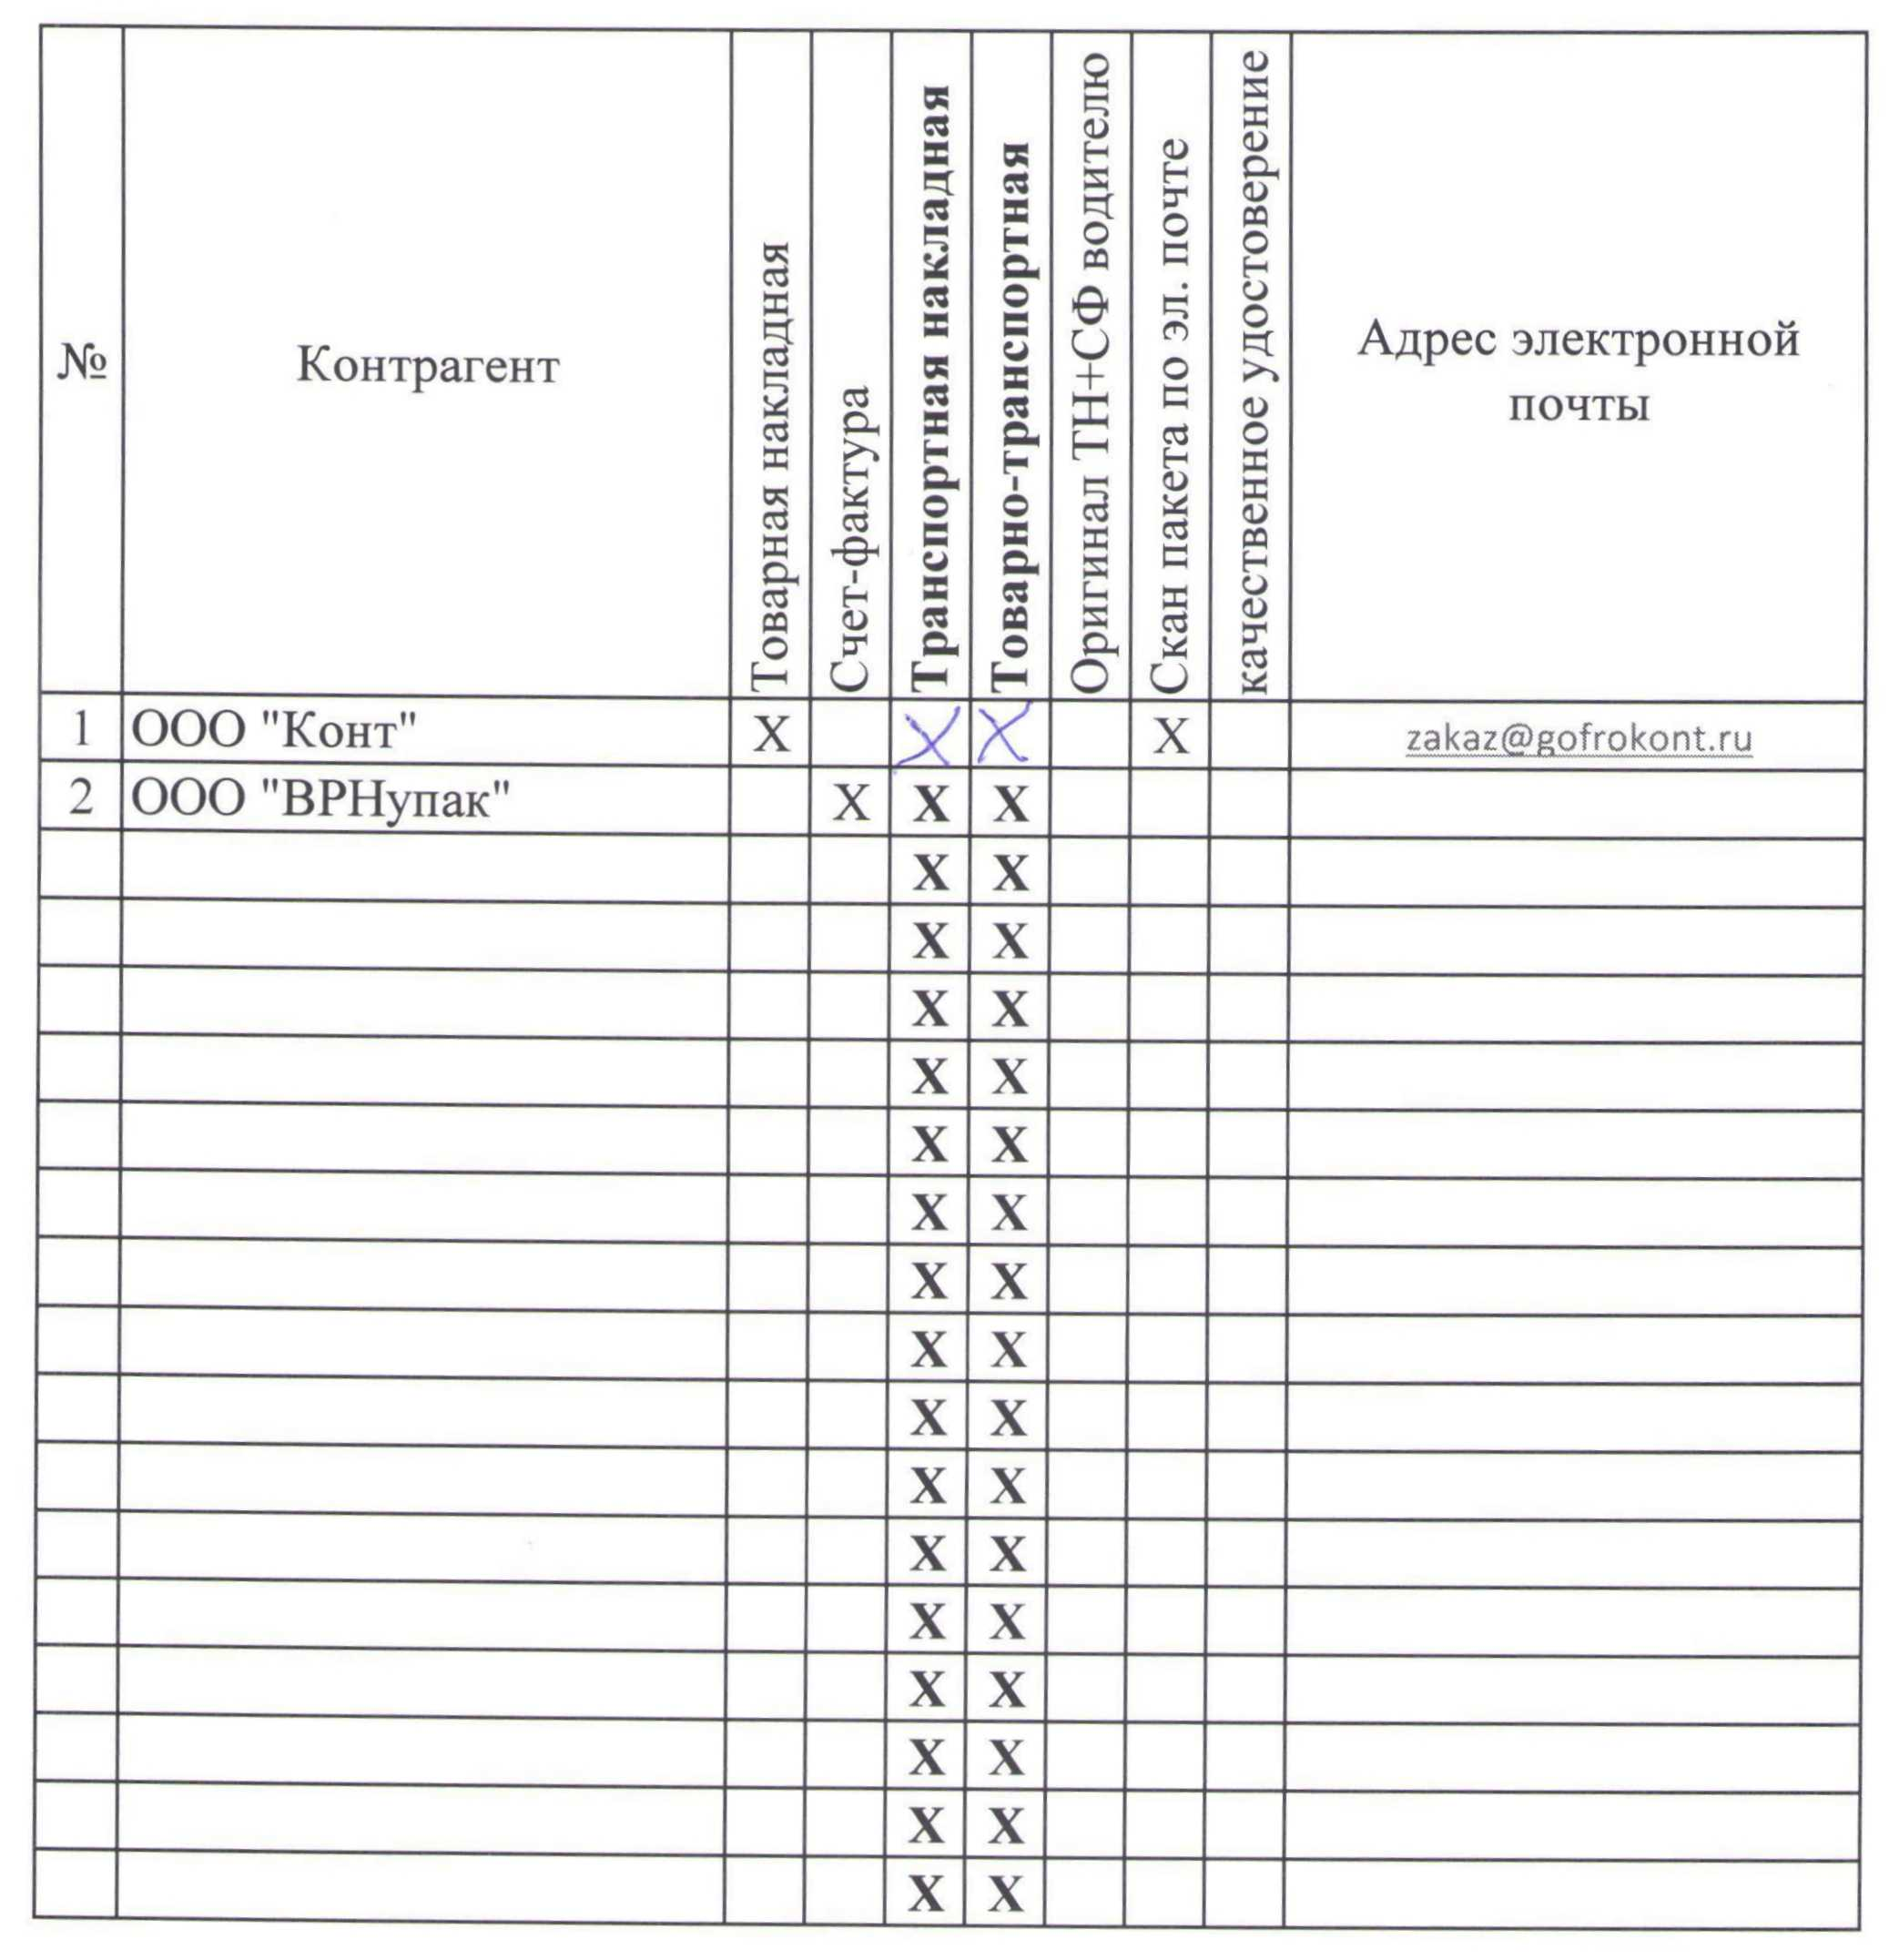
\includegraphics[width=\linewidth, height=0.94\textheight, keepaspectratio]{Pics/f12.jpg}
\end{center}
\caption{Реестр контрагентов}
\label{pic:f12}
\end{figure}

\clearpage